\documentclass[12pt]{article}
\usepackage[francais]{babel}
\usepackage[utf8]{inputenc}
\usepackage[T1]{fontenc}
\usepackage{graphicx}
\usepackage{fancyhdr}
\usepackage{hyperref}
\usepackage{float}
\usepackage{amsmath}
\usepackage[margin=1in]{geometry}
\usepackage{indentfirst}
\usepackage{titlesec}
\usepackage{appendix} 
\newcommand{\sectionbreak}{\clearpage}

%presentation of the document
\title{Projet Modélisation et Programmation Orientée Objet\smallbreak Rapport de conception\smallbreak Quatrième année - informatique }
\author{Alexandre \textsc{Audinot},  Dan \textsc{Seeruttun-{}-Marie}}
\date{17/11/2014}
\setlength\parindent{15pt}
\begin{document}
\maketitle

\begin{figure}[!h] 
\centerline{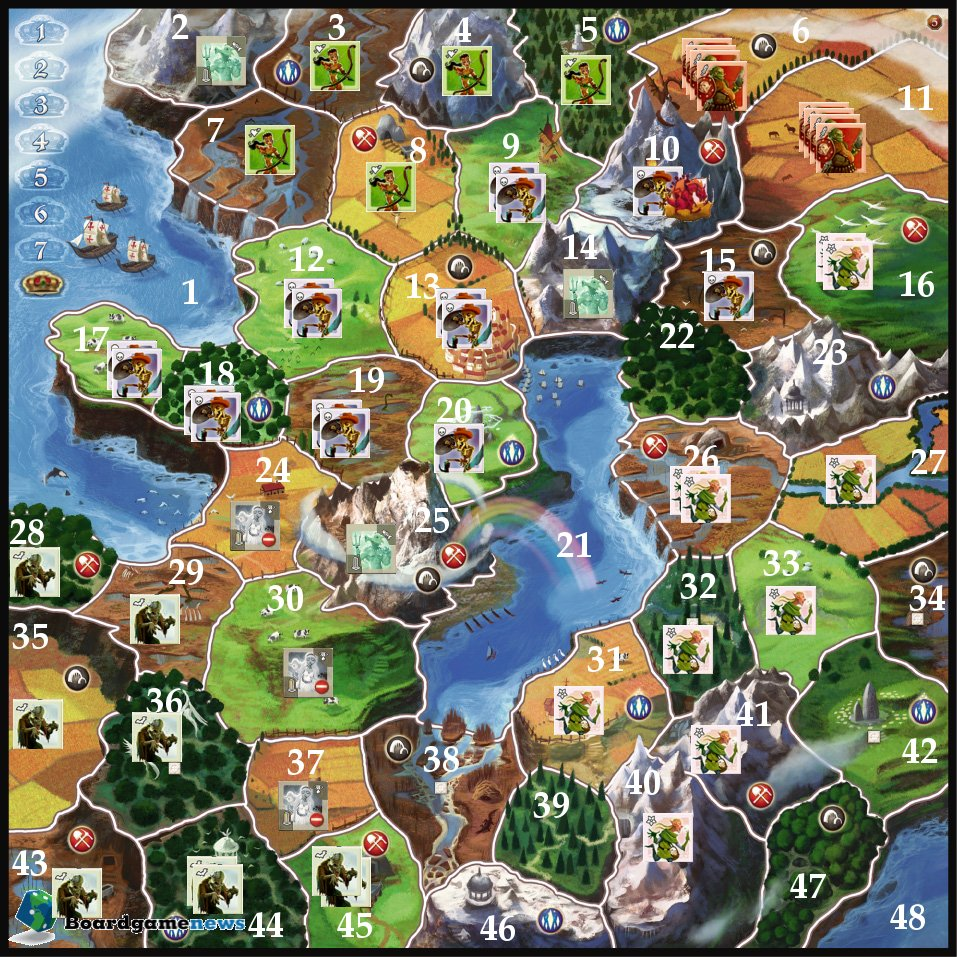
\includegraphics[scale=0.30]{img/cover.jpg}}
\end{figure}
\newpage

\newpage
%to add a table of contents
\tableofcontents
\newpage
\newpage


\section{Introduction}
\input{"intro.tex"}
\newpage
\section{Généralités sur le jeu}
\input{"part1.tex"}
\newpage
\section{Approche en détail}
\input{"part2.tex"}
\newpage
\section{Structure du code}
\input{"part3.tex"}
\newpage
\section{Conclusion}
\input{"conclu.tex"}
\newpage
\section{Annexes}
\input{"annexes.tex"}
\end{document}


